\section{Evaluations}
\label{evaluation}

In this section, we show the results of experimental evaluation of our convolutional neural networks for both Adjective Noun Pair classification and image sentiment prediction.

\subsection{Datasets}
\label{eval_datasets}

\begin{table}
		\caption{Datasets}
		\label{table:datasets}
		\begin{threeparttable}
			\centering
			\begin{tabular}{l|cccc} \hline
				Dataset & size & class & p/n & workers \\ \hline
				SentiBank-Flickr \cite{borth2013large} & ~316,000 & 1553 ANPs & N/A & auto \\ 
				SentiBank-twitter \cite{borth2013large} & 603 & 2 & 3.53 & 3/3 \\
				twitter \cite{you2015robust} & 1269 & 2 & 1.54 & 3/5\\
				Bing \cite{ahsan2017towards} & 8,812 & 3 & 2.76 & 2/3 \\ \hline
			\end{tabular}
			\begin{tablenotes}
				\item Datasets with the no. of images and no. of mid-level representations if applicable. We also list how the label is generated, the number following manual method shows how many workers label each image. There are much more positive images than negative images as people tend to engage more with positive posts \cite{kramer2014experimental}. We discard all the neutral images in all datasets.
			\end{tablenotes}
		\end{threeparttable}
\end{table}

We collect several public available data and list them in table \ref{table:datasets}. The SentiBanck-Flickr dataset is crawled from the flickr website with each ANP as keyword. All the rest datasets are manually annotated by multiple workers. Collecting data for image sentiment analysis is challenging because not only the image needs to be manually labeled, but also each image normally require multiple people to label it as it is very common for people to have different opinions on the same image. In the end, only a portion of the labeled data can be used, for example, images with all 5 annotators agree on the sentiment label. We show in table \ref{table:datasets} the number of annotators for each image of each dataset and the minimum number of workers are required to agree on the label.

Due to the size of the datasets, we use the SentiBank-Flickr dataset as our training/validation dataset, and the rest three dataset as our testing dataset. All the images are center cropped to 227 x 227 before feeding to the network. There are 1553 different ANPs in the SentiBank-Flickr dataset belongs to 530 different noun classes. 


\subsection{Experiment settings}
\label{eval_system}

We evaluate our neural network on a single server with a nVidia P5000 GPU. The learning rate of the network is set at 0.0001 for both training stages. We use a batch size of 64 and train the network for 300 epochs (first stage 200 epochs and second stage 100 epochs). The training time of 300 epochs over 316,000 images is around 3 days and the testing over all three testing sets takes less than an hour. We evaluate our CNN with triplet loss and compared the results with the CNN proposed in \cite{campos2017pixels}.

\subsection{ANP classification}
\label{eval_anp_accuracy}

\begin{table}[h]
		\caption{Five-fold cross-validation accuracy for ANP classifition}
		\label{table:anp_accuracy}
		\centering
		\begin{tabular}{l|ccc} \hline
			Model & top-1 & top-5 & top-10 \\ \hline
			Baseline CNN \cite{chen2014deepsentibank} & 14.76\% & 18.63\% & 21.47\% \\ 
			CNN w/ triplet loss & 18.33\% & 25.75\% & 29.13\%  \\ \hline
		\end{tabular}
\end{table}

We show the five-fold cross-validation results for our network after two-stage training on SentiBank-Flickr dataset in table \ref{table:anp_accuracy}. We can see that by using two-stage training with triplet loss, the ANP classification accuracy has increased for all cases. The highest increase in accuracy is the top-10 accuracy which is higher than 1.4 times the accuracy of the baseline algorithm. This shows that the two-stage learning indeed helps with the classification of the mid-level representation.

\begin{figure}[h]
    \centering
    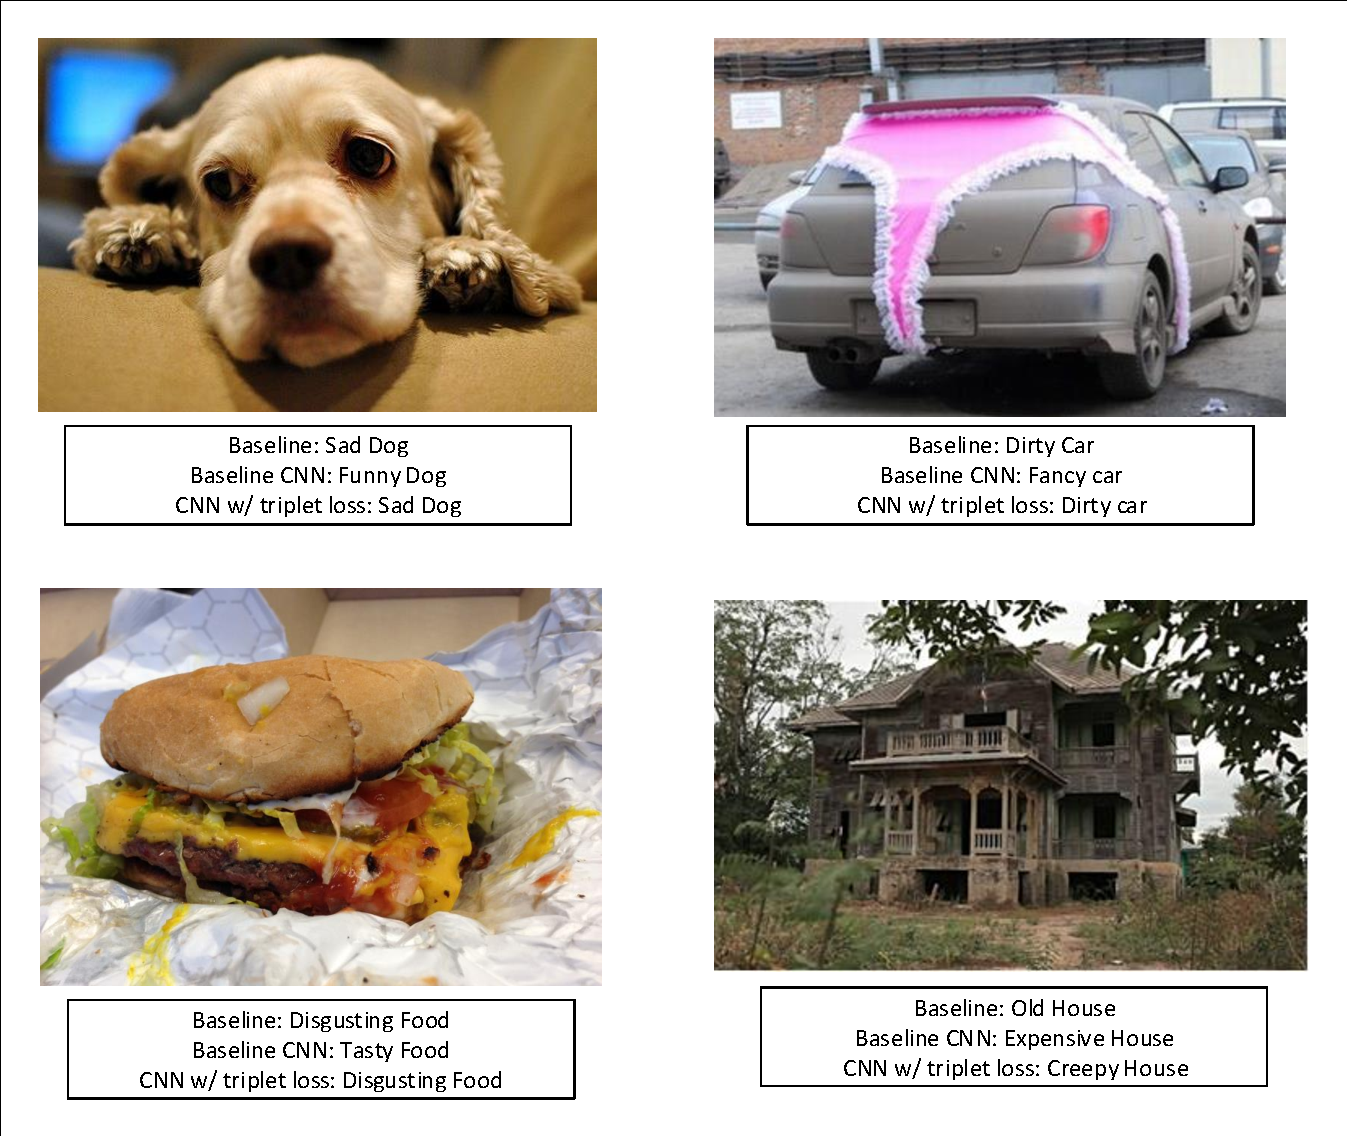
\includegraphics[width=\linewidth]{./figures/adjective_example.pdf}
    \caption{Example of CNN with triplet loss learning adjective part of ANPs}
    \label{fig:example_adj}
\end{figure}

To further show that the triplet loss can force the network to learn more on the adjective part in the ANPs, we show several examples that the baseline network failed to recognize the adjective part but our network succeeded in figure \ref{fig:example_adj}. We can see that in these selected examples, CNN with triplet loss can correctly classify the adjective part which the baseline CNN failed to do so. Even CNN with triplet loss failed to predict the correct adjective part for the "old house" image in figure \ref{fig:example_adj}, the predicted adjective "creepy" is much closer to the ground truth than the adjective "expensive" predicted by the baseline CNN.

\subsection{Sentiment prediction}
\label{eval_sent}

\begin{table}[h]
		\caption{Image sentiment prediction accuracy}
		\label{table:sent_accuracy}
		\centering
		\begin{tabular}{l|ccc} \hline
			Model & SentiBank-twitter & Twitter & Bing \\ \hline
			Baseline CNN \cite{chen2014deepsentibank} & 82.4\% & 74.1\% & 66.8\%  \\ 
			CNN w/ triplet loss & 88.3\% & 76.3\% & 73.9\%  \\ \hline
		\end{tabular}
\end{table}

We show in this section the image sentiment prediction based on the predicted ANP by our network on three different testing datasets in \ref{table:sent_accuracy}. The final sentiment prediction is made by taking all top-10 ANPs predicted by the neural network. We can see that by increasing the ANP classification accuracy, the image sentiment prediction can reach a higher accuracy. 
